% This is samplepaper.tex, a sample chapter demonstrating the
% LLNCS macro package for Springer Computer Science proceedings;
% Version 2.20 of 2017/10/04
%
\documentclass[runningheads]{llncs}
%
\usepackage{graphicx}
\usepackage{color}
\usepackage{amsmath}
\usepackage{amssymb}
\usepackage{csquotes}
\usepackage{todonotes}
% Used for displaying a sample figure. If possible, figure files should
% be included in EPS format.
%
% If you use the hyperref package, please uncomment the following line
% to display URLs in blue roman font according to Springer's eBook style:
\usepackage{hyperref}
\renewcommand\UrlFont{\color{blue}\rmfamily}

\begin{document}
%
\title{Assuring Confidence in the Perception Chain of Highly Automated Vehicles
\thanks{Funded by the Deutsche Forschungsgemeinschaft under grant number 392437295.}}
%
%\titlerunning{Abbreviated paper title}
% If the paper title is too long for the running head, you can set
% an abbreviated paper title here
%
\author{Werner Damm\inst{1} \and
Martin Fr\"anzle \inst{1} \and
Willem Hagemann \inst{1} \and
Astrid Rakow \inst{1} \and
Mani Swaminathan \inst{1}}
%
\authorrunning{W. Damm et al.}
% First names are abbreviated in the running head.https://www.overleaf.com/1268442994rnstkwtzmypt
% If there are more than two authors, 'et al.' is used.
%
\institute{University of Oldenburg, Germany \\
\email{\{damm, fraenzle, hagemann, rakow, swaminathan\}@informatik.uni-oldenburg.de}\\
}
%
\maketitle              % typeset the header of the contribution
%
\begin{abstract}
%The abstract should briefly summarize the contents of the paper in 15--250 words.
%\keywords{First keyword  \and Second keyword \and Another keyword.}
We address what is currently perceived as one of the biggest challenges in deployment of Highly Automated vehicles (HAV), by presenting a method and supportive architecture which allows to mathematically prove that the risk of misperceptions of \enquote{relevant} environmental artefacts of an HAV is less than a given level of societally accepted risk. The method requires the derivation of quality guarantees for sensors in different \enquote{Operational Design Domains (ODDs)} \cite{NHTSF}, as encouraged by the NHTSF, and proposes and exploits a range of techniques allowing to ultimately provide rigorous bounds on misclassifications for critical environmental artefacts, under the assumption, that training and test data are stochastically independent and drawn from distributions reflecting real-world traffic. This paper focusses on the presentation of the method and approach, and will be complemented by follow up publications in assessing the approach in realistic settings.
\keywords{Highly Automated Vehicles, Learning Algorithms, Safety Assurance, Perception Chain}
\end{abstract}
%
%
\section{Introduction}
\textcolor{red}{The \emph{assured autonomy} program of DARPA~\cite{AssuredAutonomy}

Assuring the safety of HAV entails assuring, that what the ego car beliefs to be true about its environment, and actual ground truth, rarely differ for all aspects which are relevant for ensuring the safety of the ego vehicle. How rare is rare enough is a matter of societal debates -- e.g. the German Department of Transportations requires HAVs to reduce the overall rate of fatalities. This paper answers the following question: if  r  is the level of societally accepted risks budgeted for misconceptions, how can we mathematically prove that perception of \enquote{relevant} environmental artefacts err at most with rate r? (We will clarify the vague term \enquote{relevant} in the text below)

We provide a mathematical setting for addressing this challenge, which is based on a reference architecture for the key functional ingredients of the perception chain. While clearly each OEM will have highly proprietary implementations, there seems to an emerging consensus in ongoing and currently prepared projects on Verification and Validation of HAVs in Germany, that an agreement on a functional reference architecture is both desirable and achievable. Our proposal for the reference architecture uses labelled occupancy grids for fusion of data from radar, lidar, video, etc, and as interface to learning-algorithms based components for classifying objects in the environment of the ego-vehicle according to a (to be standardized) partially ordered ontology. We assume that each artefact in this ontology comes with class definitions characterizing both static and – if applicable – dynamic aspects, such as e.g. ODD dependent models for typical traffic behavior (e.g. characterizing variations in lateral and longitudinal acceleration of vehicles in a neighboring highway lane, or of pedestrians in an urban pedestrian crossing), and will exploit such knowledge to reduce misclassification rates. The reference architecture also requires for each sensor the capability to identify harsh environment conditions (where no sufficiently tight bounds for risk of misconceptions can be given), and exploits this information in mechanisms for sensor fusion. The reference architecture also gives formal meaning to the vague term \enquote{relevant} environmental artefact, in that the maneuver component provides feedback to the criticality of achieving high confidence information for individual fields in the occupancy grid: errors in misclassifications of objects only count, if they relate to such critical classifications. Finally, we propose a safety net reducing likelihood of misclassifications, in declaring \enquote{blindness} for classifications, where neither the evidence for existence of an artefact a nor the evidence for absence of a is sufficiently strong – such declaration of \enquote{blindness}, if sustained over several cycles for relevant artefacts, will automatically induce minimal risk maneuvers (as does any detected usage of the HAV outside the allowed ODD).

The main result of this paper is a methodology for formally establishing bounds on the risks of misperception for artefacts labelled \enquote{critical} by the maneuver layer. This proof is composed bottom up by propagating quality guarantees along the different levels of the perception chain. We document this proof through justifications, giving for each level the reasons why the risk of misconception can be bounded. Such justifications could provide a tool for post-mortem accident analysis.

This paper is organized as follows: 
Section \ref{sec:mathmodel} defines a mathematical model of (ground truth) traffic flow in a given ODD, where observables are defined through the ontology and their associated classes. It then formalizes for a given ego car the partial knowledge the ego car acquires about its environment based on its perception chain, and refer to these as the ego car's beliefs about its environment. We then formally define the overarching safety requirement for HAVs in a given ODD, in relating the level of precision and risks of misconception between ground truth and beliefs of the ego vehicle. Section \ref{sec:refarchitecture} defines the reference architecture of the perception chain as outlined above.
Section \ref{sec:example} illustrates our proof methodology with a simple example. Section \ref{sec:proofrule} contains the formal proof rule and key elements of the underlying statistical arguments for bounding the level of risk. Section \ref{sec:relatedwork} discusses related work. We wrap up with a way forward in using this methodology.



\section{Mathematical Model}\label{sec:mathmodel}
We assume as given a partially ordered ontology $O = (A, <)$ containing all relevant environmental artefacts for HAV. Initiatives towards identification of such an ontology are currently part of a number of R\&D projects on HAV, including the PEGASUS project\footnote{\url{www.pegasusproject.de}}. The ordering relation reflects the degree of precision of classification of objects, with $\bot$ (read: bottom) representing inconsistency, and $\top$ (read: top) denoting zero knowledge. The ontology contains different kinds of artefacts, e.g. relating to weather conditions (foggy, rain, snow, \ldots), road configurations (x-lane highway, T-type x lane intersection, \ldots), road conditions (dry, icy, aquaplaning, \ldots), roadside infrastructure (traffic signs, traffic lights, \ldots), traffic participants (car, truck, bicycle, pedestrian, animals, obstacles, \ldots), and surroundings of road segments (trees, buildings, \ldots). Objects in different categories are related by relations, and form separate sublattices, which are turned into a complete lattice by introducing a new top element. In this paper we will only refer to weather conditions, traffic situations, and traffic participants. Such ontologies are today in regular use as semantic basis for driving simulators such as \ldots. Sample ordering relations in the category of traffic participants are shown in Fig. \ref{fig1} below.
\begin{figure}
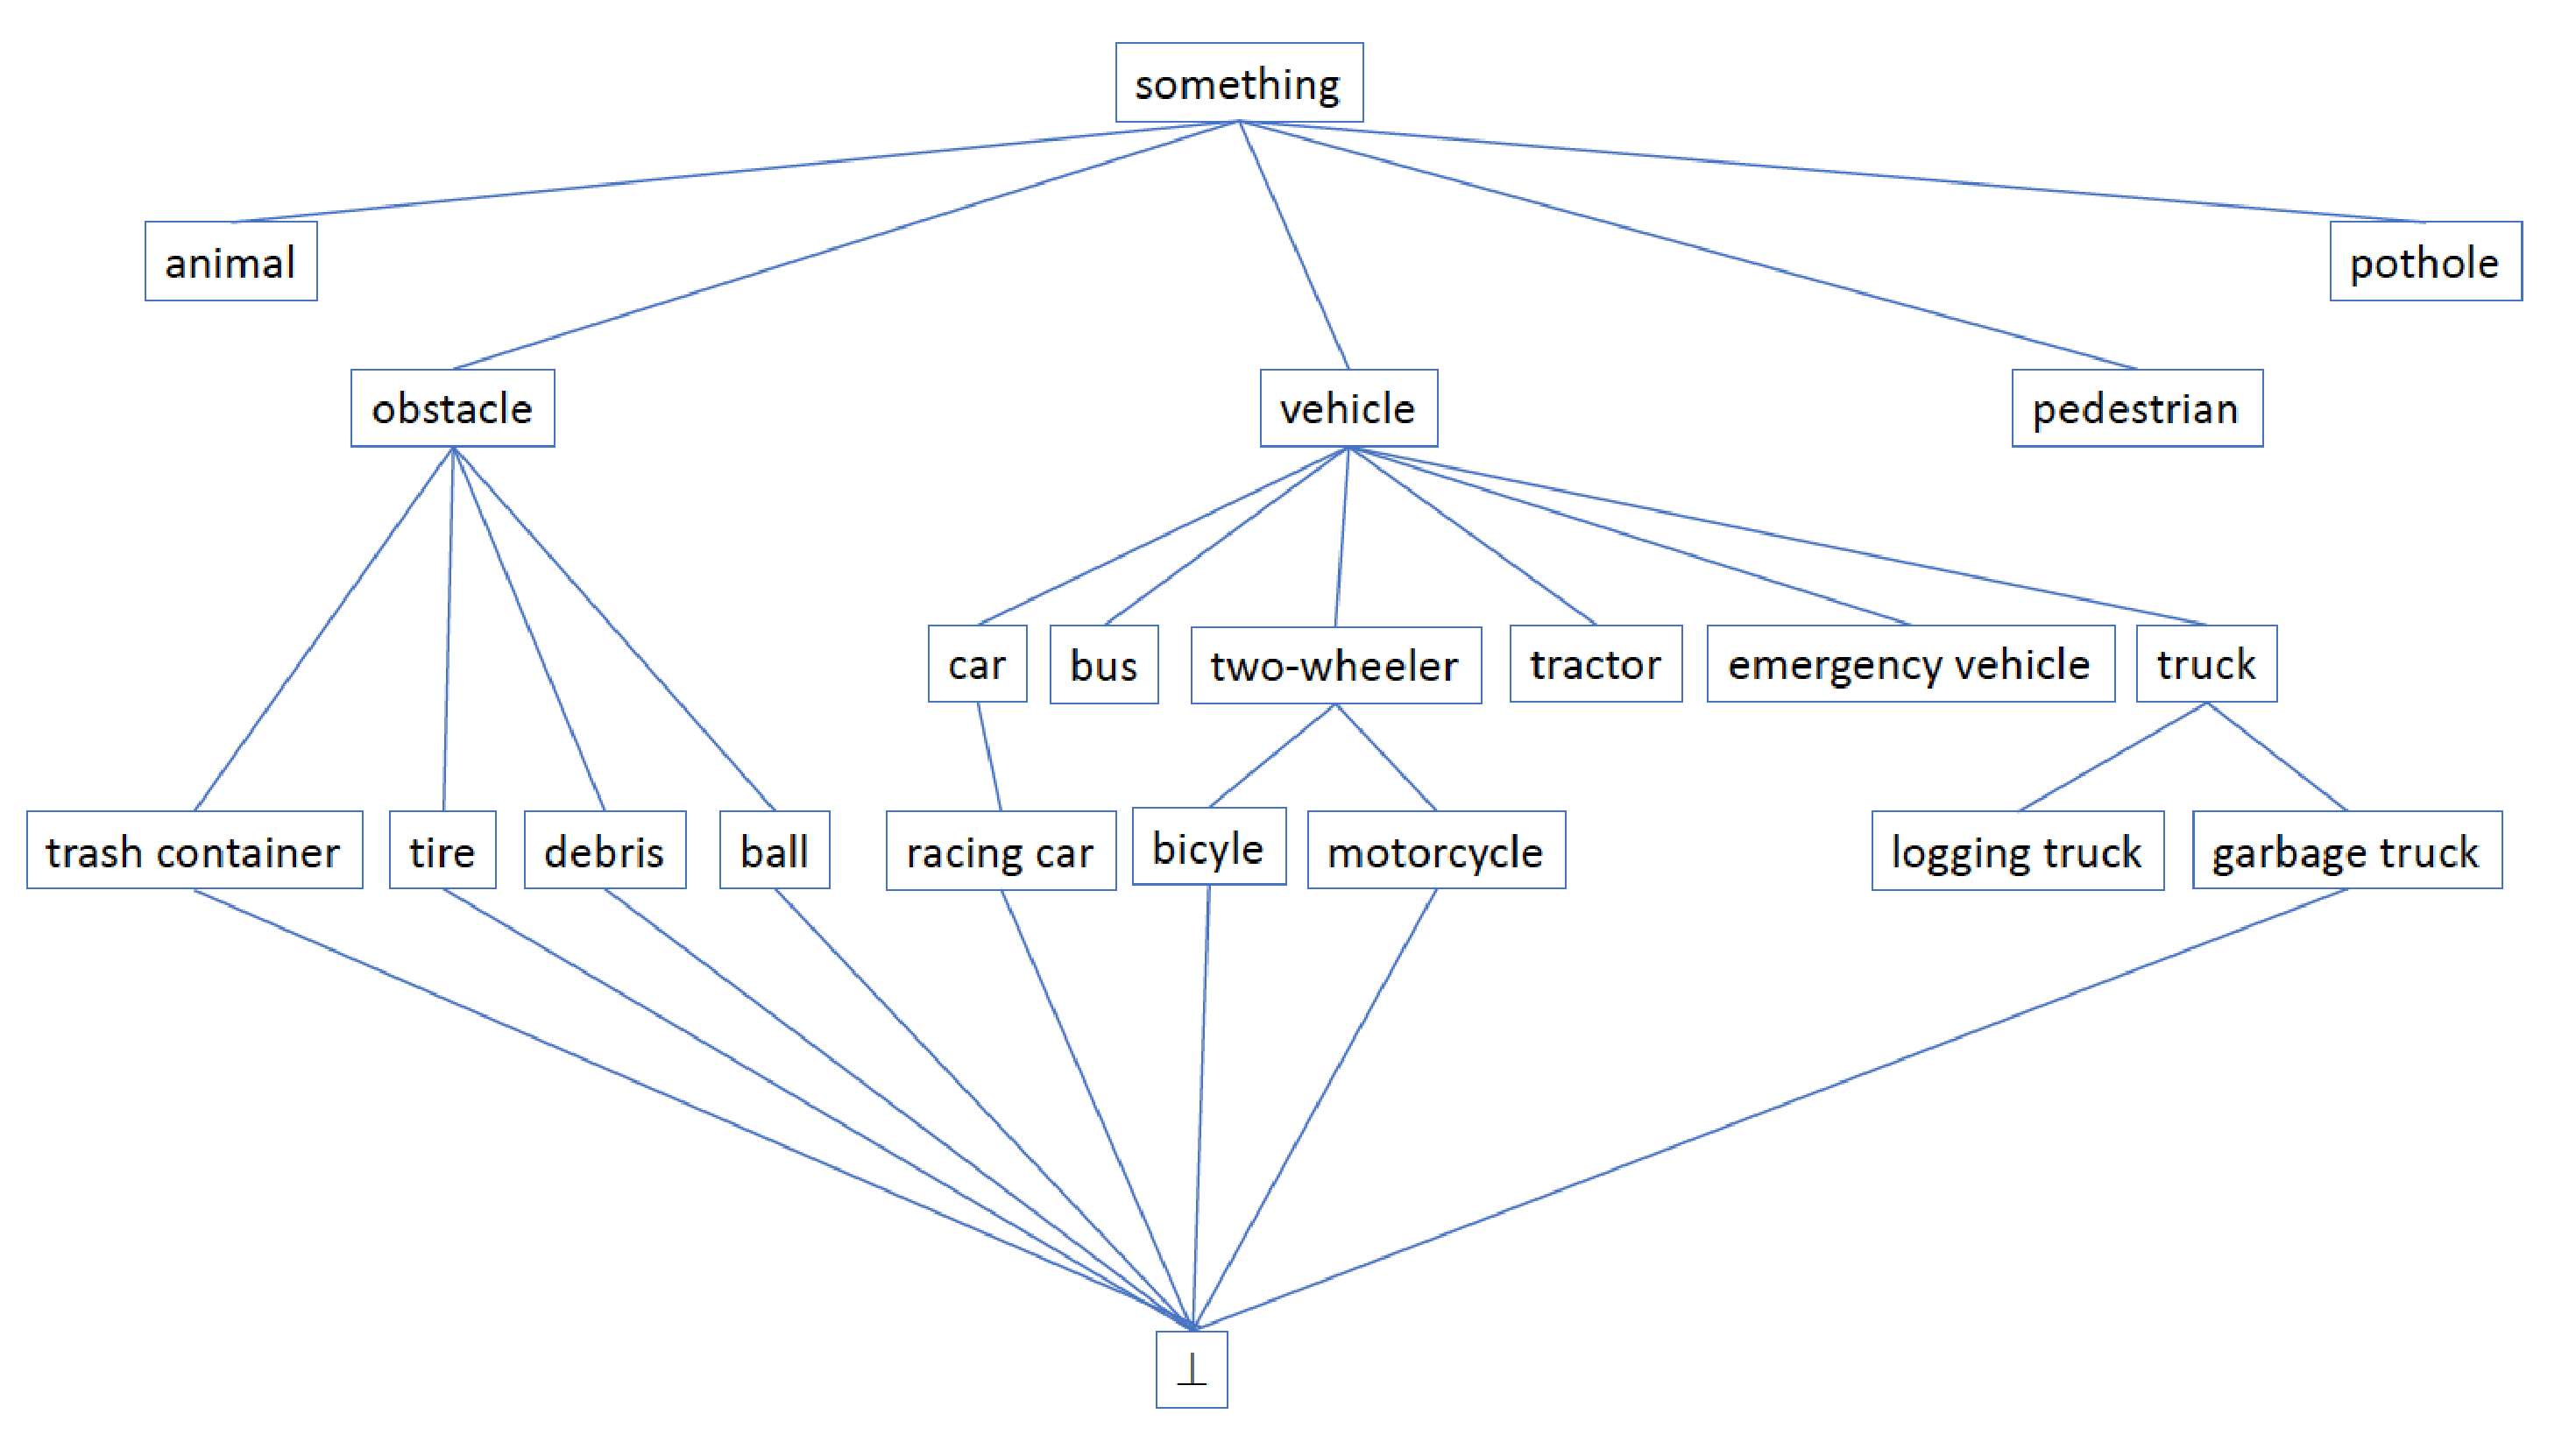
\includegraphics[width=\textwidth]{fig1.eps}
\caption{\textcolor{blue}{Sample ordering relations in the category of traffic participants}} \label{fig1}
\end{figure}

With each artefact  a  in the ontology, we assume as given a specification of its safety related aspects through a class definition cl(a). For artefacts of type road configurations, this includes specification of all geometric aspects including slope, number of lanes, width of lanes, etc. Road configurations are built from segments of a parametrized length. An operational design domain ODD is defined by constraints on types of road configurations, and constraints on prevailing weather conditions and road conditions. For each artefact veh of type vehicle, attributes of cl(veh) include the type of an instance of class road configuration, on which the vehicle is currently located, as well as its position, such as its longitudinal and lateral position on some lane of this instance of class road configuration. Moreover, each vehicle maintains its beliefs about its environment in appropriately typed attributes. Figure 2 below depicts the beliefs of ego driving on a country road: it beliefs the road surface is dry, that there is an obstacle in 250 m distance ahead blocking the lane, and that some vehicle of unknown type is approaching on the opposite lane. Importantly, cl(veh) contains as well a characterization of ODD-dependent dynamics of veh. We assume that these are given by probabilistic hybrid automata (cite \ldots), where mode changes are triggered based on believed changes of road configurations, weather conditions, road conditions, and observations of surrounding traffic and roadside infrastructure, and refer to this as pha(veh). A key point to be exploited is, that behavioral models are increasingly unconstrained along the generalization hierarchy: e.g. for class vehicle, the associated probabilistic hybrid automata is constructed from those of the next level of specialization by introducing a new start state, branching non-deterministically into the entry states of the pha's of cars, two-wheelers, trucks, emergency vehicles, etc. Similarly, we assume such models for pedestrians, animals, obstacles etc.

\begin{figure}
    \centering
    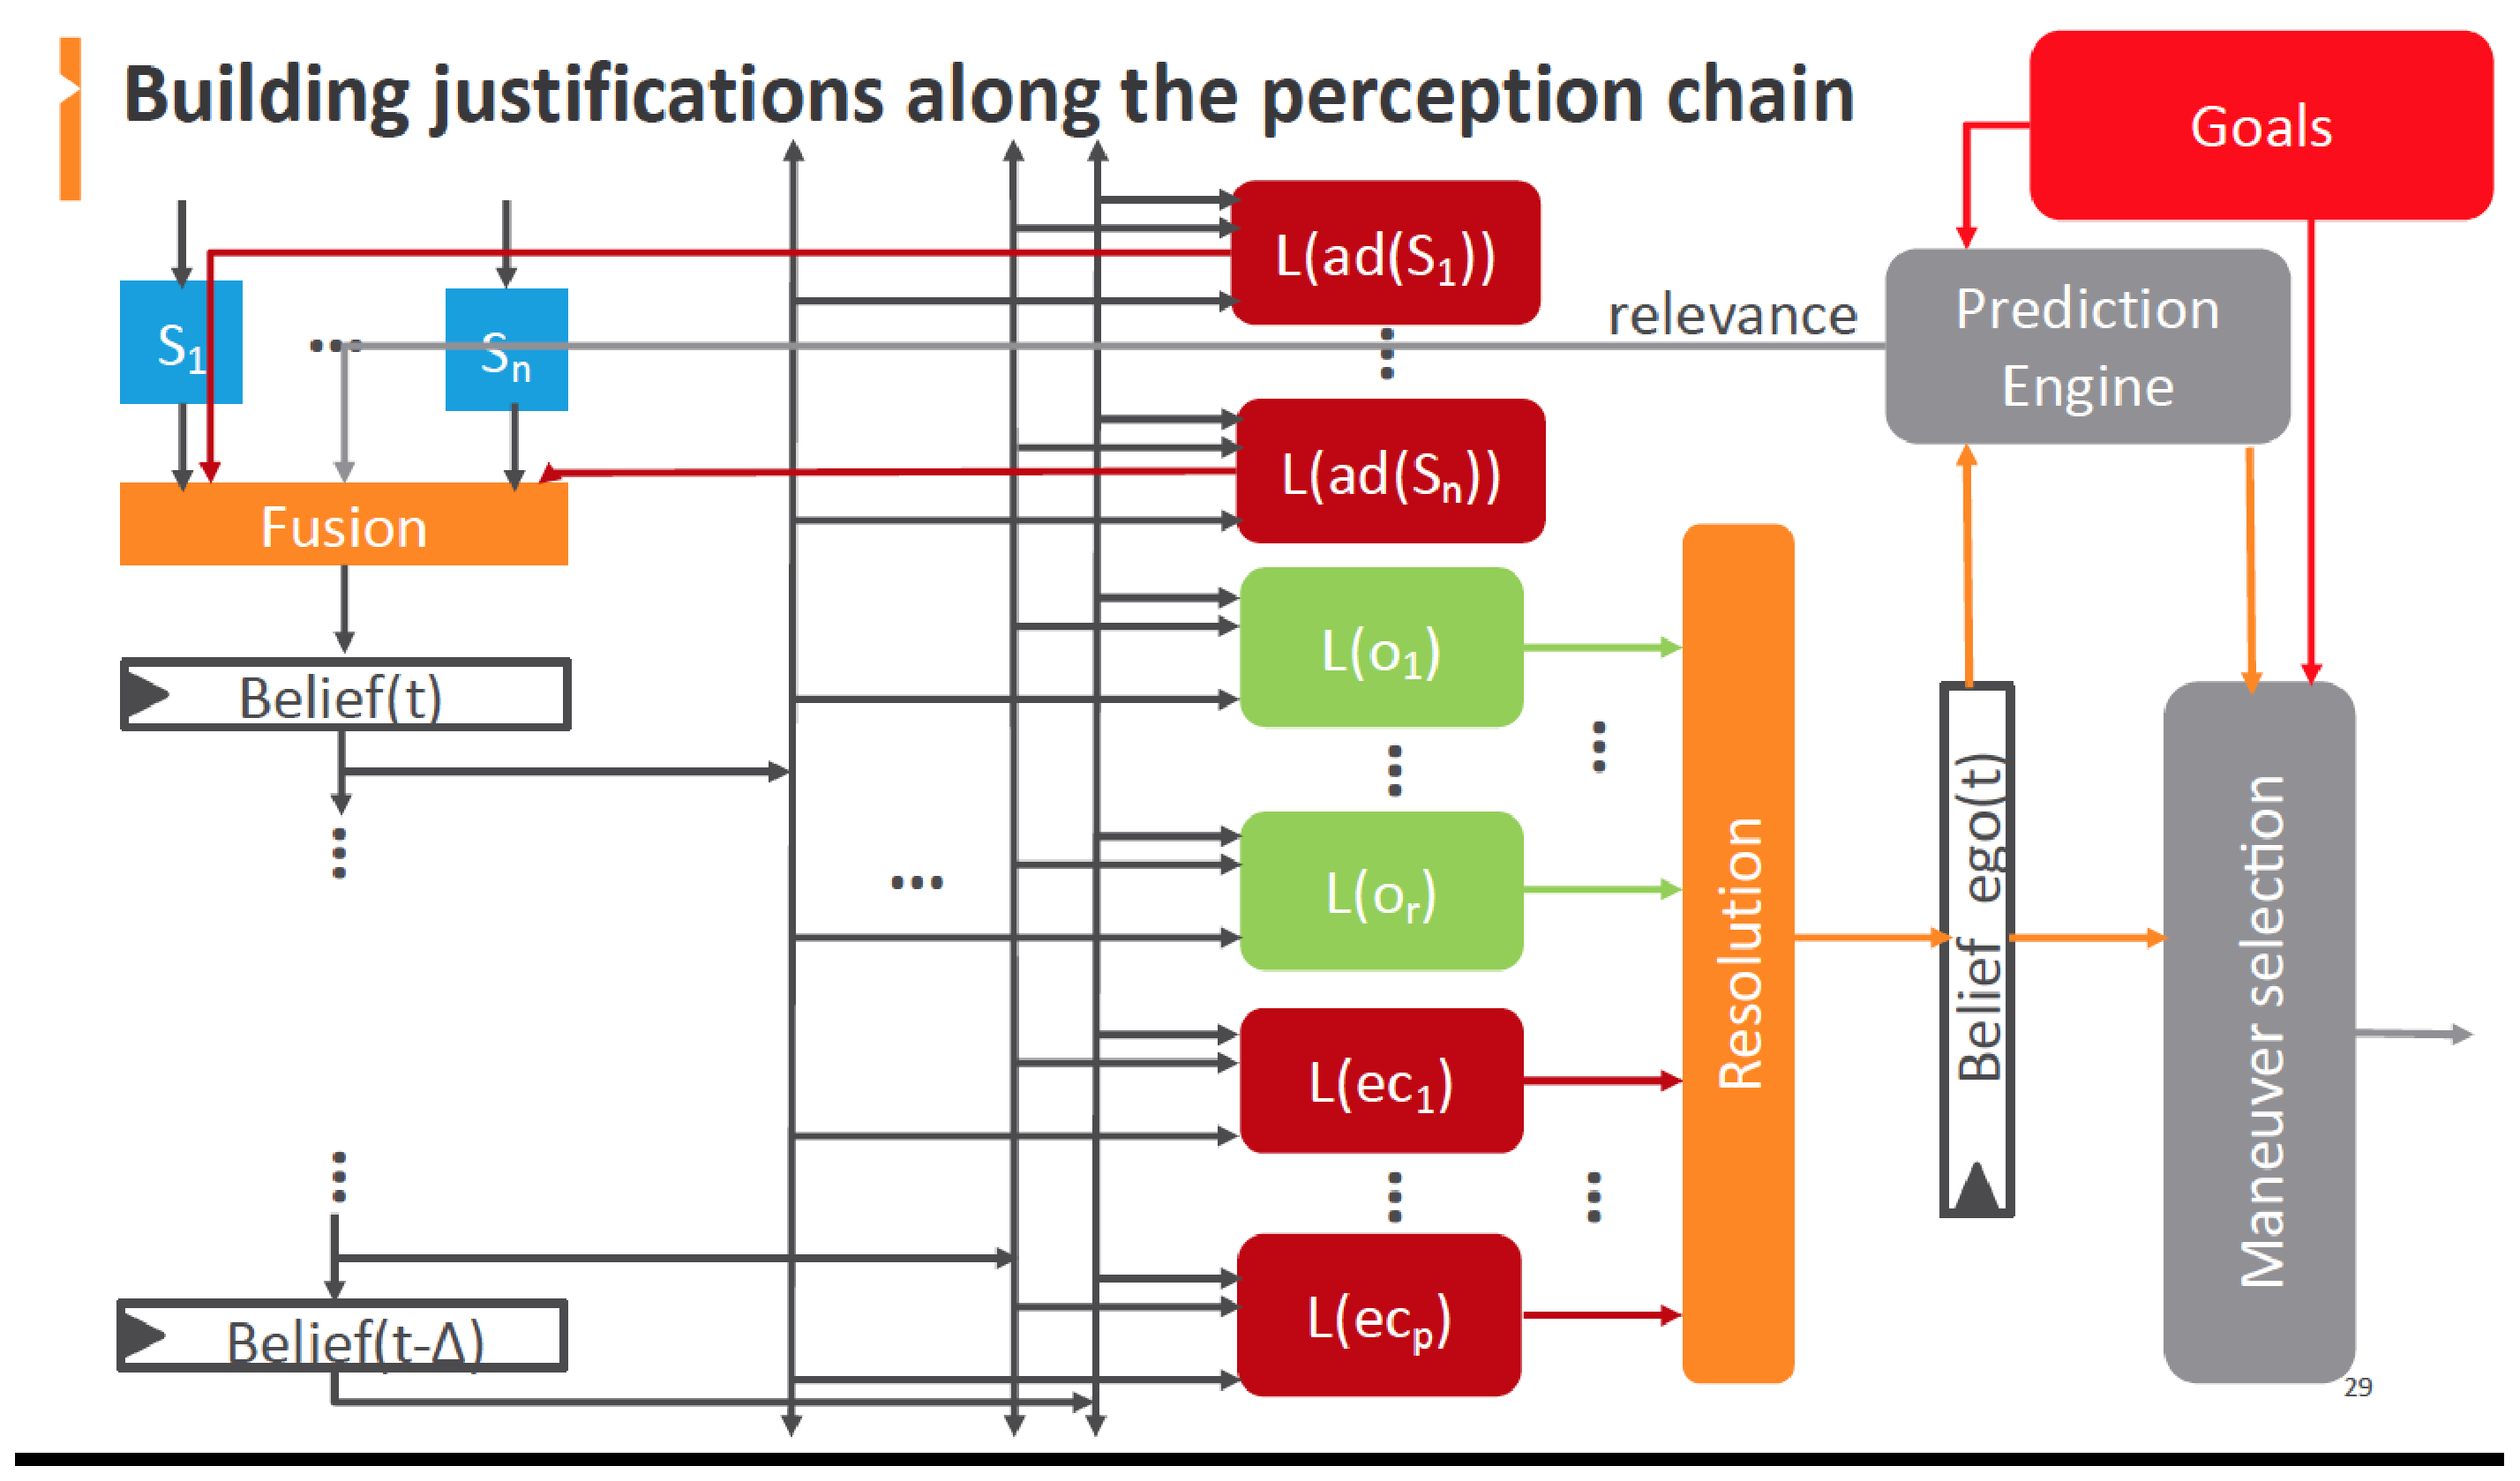
\includegraphics[width=\textwidth]{fig2.eps}
    \caption{\textcolor{blue}{Caption}}
    \label{fig2}
\end{figure}

Based on this, we can define a mathematical model of traffic evolution from the perspective of a given ego-vehicle. We define the electronic horizon of the ego vehicle to be the best-case range of perception of its on-board sensory system, and for simplicity of exposition in this paper assume this to be given by a rectangle aligned to the current pose of the ego vehicle centered at the geometric center of the ego vehicle. We call back- resp. front-horizon of ego the uttermost road segment still visible behind resp in front of the car through its electronic horizon. The mathematical model is an infinite state transition system, whose state space is constructed as follows:
\begin{itemize}
\item It contains for each point in time t  all instances of road segments extending from the instance on which the ego car is currently positioned within its electronic horizon;
\item For each of the above road segments, it contains for time t  position and speed of all vehicles on the road segment, as well as road conditions and weather condition, positions of pedestrians, animals, obstacles, etc.
\end{itemize}
The (dense time) transition relation of the mathematical model is constructed as follows:
\begin{itemize}
\item New road segments are generated at the front- and lateral horizons by randomly instantiating new instance of class road segments while obeying the constraints of the ODD.
\item These new road segments are randomly attributed with road conditions and weather conditions observing consistency constraints and physical laws, and randomly filled with vehicles of randomly chosen type, with speeds and relative distances compliant to real observed traffic flow under the given ODD.
\item Where applicable, pedestrians are positioned randomly on newly generated road segments, observing traffic rules and dynamic models of pedestrians
\item Evolution of instances of objects of classes vehicles, pedestrian, animals follow the associated dynamic models
\item The evolution of the ego-vehicle follows the driving strategy determined from its beliefs about its environment as given by a probabilistic hybrid automaton.
\end{itemize}
We refrain for space reasons from giving the formal definitions, and refer to this transition system by \textit{TS(ego)} . A state of \textit{TS(ego)} is given by a valuation of all its observables. A run of \textit{TS(ego)} defines for each observable its evolution over time, thus including trajectories of all vehicles, pedestrians, animals, obstacles within ego's electronic horizon, including the evolution of the beliefs of the ego vehicle, and the evolution of its perceived road segments. We call \textit{RUNS(TS(ego)}) the set of all runs of \textit{TS(ego)}.

We can now formalize the meta requirement for the quality of the perception chain, up to the not yet formally defined notion of relevance, in a probabilistic linear time temporal logic, with observables defined by valuations of all attributes of all instances of classes within the electronic horizon of ego, over a typed first-order signature induced by the types of attributes in the ontology. Ideally, for each point in time, the ground truth of all relevant artefacts in ego's electronic horizon, in particular position and speed of surrounding traffic participants, road- and weather conditions, coincide exactly with ego's beliefs about these artefacts. We must relax this unachievable ideal first by considering standard measurement errors, and allowing classifications to be vague, as long as they are correct with respect to the ordering relation in the ontology, i.e. the ground truth classification is a specialization of the believed classification. Third, misclassifications and misperceptions will occur, but we want these to be bounded by the societally accepted level of risk. Assuming for each artefact $a$ a metric $d_a$ to measure the distance between ground truth and beliefs of $a$, and a safe level of measure tolerance $\delta_a$ we want almost always these to be consistent for a minimal time period $\Delta$ sufficient to take safe maneuver decisions for the HAV. This leads to the following formal requirement on the confidence of the perception chain of the HAV vehicle ego:

$\textit{Safe\_perception}(ego) = \forall a \in \textit{observables}(\textit{TS(ego)}):  \Box (\textit{relevant}(a) \Rightarrow$\hfil\\ $P(\Box_{\leq\Delta}d_a(a, \textit{belief}(a))> \delta_a) < r)$.

We will now propose methods to establish that \textit{TS(ego)} meets this overarching safety requirement. To this end, we will first introduce architectural constrains enabling such proofs, as expressed in the reference architecture of the perception chain elaborated in the next section.




\section{The functional reference architecture of the perception chain}\label{sec:refarchitecture}
This section develops a functional reference architecture for the perception chain allowing to provably bound the risk for misperceptions. The following principles guided this proposal:
\begin{enumerate}
\item It must be possible to bound the contributions to risks for each component of the perception chain.
\item This entails the need to specify for each element in the perception conditions under which this element can be \enquote{trusted}. Violations of such conditions must be monitored and -- if persistent -- must induce declaration of \enquote{blindness}, automatically inducing minimal risk maneuvers.\todo{Ist das "blame principle" von MobilEye ein Minimum Risk Maneuver? Es erlaubt eine wuenschenswerte Art von Blindness...}
\item The reference architecture must provide guidance as to the degree of precision of perception required for current maneuver decisions.
\end{enumerate}
We discuss the implications of these design principles in separate subsections, along the flow through the perception chain.

\paragraph{Quality criteria for sensor components}

While radar systems are widely deployed for variants of ACC systems and emergency breaking system, their integration in level 3, 4, or 5 HAVs constitutes a completely different operational context, because the overall safety case can no longer rely on human supervision of the environment of the ego car. Well known phenomena such as ghost objects stemming from undesired and uncontrollable reflections, or \enquote{stealth type cars} such as the VW beetle, or simply reflections induced by metal-coating of truck planes are but examples of a plethora of phenomena, which all influence quality of object detection through radar. With the transition to level 3, 4, 5 systems, quality criteria must take a more rigid form: we must be able to quantify the risks of missing objects, or showing ghost objects. Similar types of distortion of perception are well known and documented for Lidar systems in certain types of rain conditions, for video systems in certain types of lighting conditions, etc. We propose a uniform quality measure for different type of sensor systems, by assessing their capability to contribute to detecting all relevant objects in the what is often called the occupancy grid enclosing the ego car. Specifically, we take a suitable 3d extension of the electronic horizon of the ego vehicle, and assume a sufficiently fine grained, not necessarily homogeneous partitioning of this 3d space, and refer to this as \emph{occupancy grid(ego)}. We view sensors as providing labels of the partitions of the occupancy grid, providing information about whether a given sensor has identified some artifact in this grid partition, depending on sensor type filled with additional information such as speed (for radar), temperature (for infrared), gray-scale distribution of pixels for video cameras, \ldots, typically as distributions with confidence levels, e.g. regarding the likelihood of some artifact being located in this grid partition. The formal quality requirement is just an instantiation of the safe perception requirement in formula (1). Specifically, for a given position \textit{pos}  of sensor  \textit{s}  on vehicle ego, let us denote by \textit{visible(s,pos)} the coherent subspace of the occupancy grid covered by sensor \textit{s} when mounted at this position, then for any relevant artifact  $a$, and any property  \textit{label($a$)} discernable by  \textit{s}  in this position, we would want the sensor \textit{s} to almost always, up to some bounded risk $r_s$, correctly label the grid field with \textit{label($a$)} at time $t$, when $a$ is at a visible grid partition in ground truth, as determined by the state of \textit{TS(ego)} at that point in time:

\begin{align}\label{eq:safelabelling(s,pos)}
    \textit{Safe}\_&\textit{labelling(s,pos)} \equiv 					\\		
 & \forall a\in\textit{ observables(TS(ego))}\forall p \in \textit{occupancy grid(ego)}:\nonumber\\  
& \Box (\textit{relevant}(a) \land a \textit{ is at } p\land p\in \textit{visible(s,pos)} \nonumber\\
& \Rightarrow P(\neg( \Box_{\leq\Delta} d_{a,s}(a,\textit{label}(a))\leq\delta_{a,s}))) < r_s\nonumber
\end{align}

Since phenomena such as reflections discussed above will have strong negative impact on achieving sufficiently precise distances between beliefs and ground truth, we propose to characterize for each sensor adverse conditions. Only by separating out such conditions can we obtain a sufficiently tight bound on the risks of incorrect labelling of the occupancy grid, to achieve an overall risk tolerated by society. The down side is the need to then also identify reliably such adverse conditions; in this paper, we integrate such adverse conditions in our ontology, and then use the full power of the perception chain to learn sufficiently reliable classifications of adverse conditions, see next subsection. As in \cite{galbas}, we propose to use learning techniques from field observations to characterize adverse conditions for each sensor \textit{s} and to derive such quality guarantees. We now weaken formula (2) by weakening the criteria for sufficient precision of beliefs in that no promises regarding precision are made when adverse conditions ad occur:

\begin{align}\label{eq:safelabelling(s,pos,ad)}
\textit{Safe}\_&\textit{labelling(s,pos,ad)} \equiv\\  			
&\forall a\in \textit{observables(TS(ego))}\forall p\in\textit{occupancy grid(ego)}\nonumber:\\
&\Box(\textit{relevant(a)} \land a\textit{ is at p }\land p\in\textit{visible(s,pos)} \Rightarrow\nonumber\\
&P(\neg(\Box_{\leq\Delta} (d_{a,s}(a, \textit{label(a)})\leq \delta_{a,s}))\textit{ unless } ad)) < r_s\nonumber
\end{align}

Note that we can in particular encode the constraints of a given ODD in such adverse conditions, which thus entails that information of a sensor is not trusted if working outside the constraints of the ODD. OEMs compensate weaknesses of types of sensor systems by providing redundancy and diversity and using sensor fusion. We can derive a composed sensor s from fusing two qualified positioned sensors $<$s1,pos1$>$  and $<$s2,pos2$>$ to system s as follows:
\begin{itemize}
\item ad(s) is the disjunction of ad(s1) and ad(s2)
\item visible(s) = visible($<$s1,pos1$>$) $\cup$ visible($<$s,pos2$>$)
\item for each p\in \textit{occupancy grid(ego)}:  \\
if p $\in$ visible($<$s1,pos1$>$) $\cap$ visible($<$s2,pos2$>$) then
\begin{itemize}
\item if $\neg$ad(s1)$\land\neg $ad(s2) then\\
if label(s1)(p) $\land$ label(s2)(p) $\not=$ false 
\begin{itemize}
\item[] then label(s)(p) := label(s1)(p) $\land $label(s2)(p)
\item[] else label(s)(p) := $\bot$
\end{itemize}\todo{Weiss nicht wie man es besser machen soll, aber die Nichtmonotonie, dass man hier im besser informierten Fall pessimistischere Label zuordnet als wenn ein Sensor erblindet ist, stoesst mir auf.}
\todo[inline]{WH: das letzte if--then--else l\"asst sich zu "label(s)(p) := label(s1)(p) $\land$ label(s2)(p)" zusammenfassen (da $\bot$ ja gerade false repr\"asentiert).}
\item[] else if ad(s1) )$\land\neg$(s2) then label(s)(p) := label(s1)
\item[] else if $\neg$ad(s1)$\land$ad(s2) then label(s)(p) := label(s2)
\item[] else if ad(s1) $\land$ ad(s2) then label(s) := $\bot$
\end{itemize}
\item[] else if p$\in$visible($<$s1,pos1$>$) $\setminus$ visible($<$s2,pos2$>$) then\\	
if $\neg$ad(s1)
\begin{itemize}
    \item[] then label(s) := label(s1)
	\item[] else if ad(s1) then label(s) := $\bot$
	\end{itemize}
	else if p $\in$ visible($<$s2,pos2$>$) $\setminus$ visible($<$s1,pos1$>$) then
	\begin{itemize}
	\item[] if $\neg$ad(s2) 
	\begin{itemize}
	    \item[]then label(s) := label(s2)
	\item[] else if ad(s2) then label(s) := $\bot$
    \end{itemize}
    \end{itemize}
\end{itemize}
Note that any detected inconsistencies are marked $\bot$. Also the combined sensor labels fields p with $\bot$ if p is only visible for one sensor, but this sensor cannot be trusted because of prevailing adverse conditions. We derive quality guarantees for sensor fusion in Section \ref{sec:proofrule}. For observations where both sensors are in non-adverse conditions, and both sensors observe p, then the risk of misclassifications is reduced to $r_{s1} \times r_{s2}$ if we can prove that misperceptions are stochastically independent under operating conditions favorable for both sensors, otherwise the risks for misperception of the fused systems for fields p visible to both sensors is min($r_{s1}$,$r_{s2}$).

Level 4 and 5 HAVs must guarantee by construction sensor completeness with maximal risk r: for all points in time, and all relevant fields p of the occupancy grid, there must at least be one positioned sensor operating in non-adverse conditions, such that p is visible for this sensor, and the risk of misperception by this sensor is smaller than r, unless there are multiple positioned sensors all operating in non-adverse conditions, which are stochastically independent under such conditions; in this case the products of their risk levels must be smaller than r. Since this property is more easily expressed using the formula derived in Section \ref{sec:proofrule} for sensor fusion, we formalize this key requirement of sensor completeness in Section \ref{sec:proofrule}.

\paragraph{The functional reference architecture}


Figure 3
Figure 3 shows the proposed functional reference architecture of the perception chain, where belief(t) represents the labelled occupancy grid resulting from fusion of sensors s1 to sn, as discussed in subsection A. We distinguish these from the complete reconstruction of the environment of the ego car, belief(ego), and assume that for each artifact  a in the ontology we have a dedicated learning component  L(a) for detecting both presence and absence of a in fields of the occupancy grid, see below. Note, that we assume that the prediction engine provides feedback about the relevance of fields in the occupancy grid, based on knowledge about the current beliefs of the ego car, and its current goals. Note also, that the learning components for identifying adverse sensor conditions are fed backwards into the sensor fusion unit. We propose the following measures to reduce the error of misperception:

1) To be able to exploit physical laws to optimize the prediction rate, we propose to maintain copies of such beliefs over some time window , and feed this into the classification network. This supports both object tracing as well as detection of misclassification in the resolution phase, since e.g. a pedestrian can not cross a four-lane street in one second.
2) We require for each learning component L(a) and each position in the electronic horizon to output both strength of beliefs for presence and for absence of a. We will only pass on classification votes of L(a) into beliefs of ego in the resolution process, if such strength values are separated by a safety margin determined in the validation phase of L(a), ensuring full separation for all test points.\todo{Letztlich muesste das doch bereits die Ontologie erledigen: Hier muesste doch ggf. sofort $\bot$ herauskommen.}
3) We use the ordering relation of the ontology to detect misclassifications in the resolution phase. E.g. identifying simultaneously a car and a pedestrian and the same location is impossible, unless both a car and a pedestrian where within reach to this location in the previous belief, taking into account the laws of physics capture in the respective behavioral models. Similarly, we detect inconsistencies in classification for ordered elements in the ontology, e.g. identifying a racing car by claiming that the same location does not contain a car.
4) We propose in-the-field learning for adverse conditions, by constantly comparing the individual sensors perception of the occupancy grid with the result from sensor fusion, including detection of inconsistencies. Under current regulation, such an on-line learning process must be done on a separate copy of the network and subjected to off-line verification and validation before activating it.

>>>> space permitting, I could still give an operational characterization of the resolution operator at this point: >>>>This is non-trivial, because if will have to argue about the reach set, and needs to trace objects through time

Section 5 will show how quantify the risk of misperception, by incrementally working from the guarantees of type (3) for individual sensors, through sensor fusion, through the classification network, to the resolution stage, considering the above features for detecting inconsistencies.


Werner with some help to be determined\\
3 pages	concluded at page 7,5\\
nur die Abweichungen zu diesem Bild die wir in den letzten beiden Runden besprochen haben

\section{A simple example}\label{sec:example}
Astrid\\
1 page		concluded at page 8,5

\section{Assuring Safe Perception}\label{sec:proofrule}
%Willem and Martin\\
%4,5 pages	concluded at page 13\\
\subsection{Classifier Analysis}
An ontology $\mathcal O=(\mathcal L,\sqcap,\sqcup)$ is a complete distributive lattice over a set $\mathcal L$ of labels. The unique complement of $l\in\mathcal L$ is denoted by $\overline l$. The induced non-strict partial order of $\mathcal O$ is denoted by $\sqsubseteq$ and its strict variant by $\sqsubset$. We say that a label $l\in\mathcal L$ is more specific (broader) than a label $l'\in\mathcal L$ if $l\sqsubset l'$ ($l'\sqsubset l$, respectively). A classifier $c_l$ for the label $l\in\mathcal L$ takes an artifact $a$ as input and returns a numerical value $c_l(a) \in [\min,\max]$ which corresponds to its degree of conviction that the artifact $a$ is of type $l$.
Given the upper threshold $g_l^+$ and the lower threshold $g_l^-$ with $g_l^+\geq g_l^-$ we define the label assignment for an artifact $a$ as follows
\begin{gather*}
    \Label(c_l,g_l^+,g_l^-)(a) = \left\{
    \begin{array}{ll}
    l & \text{ if } c_l(a) \geq g_l^+\\
    \overline l & \text{ if } c_l(a) < g_l^-\\
    \top & \text{ otherwise.}
    \end{array}\right.
\end{gather*}
We use the short notation $\Label(c_l)(a)$ when the thresholds are fixed. 

There are various quality measures for classifiers. A classifier is evaluated against a given a test data set $T$, where $T$ is a set of correct and complete labeled and representative set of artifacts. Hence, for each label $l\in\mathcal L$, we obtain a partitioning of $T=T(l) \cup T(\overline l)$ into the set $T(l)$ of artifacts which are labeled with $l$ and its complement $T(\overline l)$. The number of elements is denoted by $n_l$ and $n_{\overline l}$, respectively.

To analyze a classifier $c_l$ we are mainly interested in the relation between the threshold $g_l^+$, the true positive rate (\TPR), and the false positive rate (\FPR) on the one hand, and the relation between the threshold $g_l^-$, 
the true negative rate (\TNR), and the false negative rate (\FNR) on the other.
For each classifier we obtain two ROC curves (receiver operating characteristics):
\begin{itemize}
\item ROC curve $RP$ represents the relationship of $\TPR(g_l^+)$ and $\FPR(g_l^+)$,
where
\begin{gather*}
    \TPR(g_l^+) = \frac{ | T(l) \cap \{ c_l(a) \geq g_l^+ \}|}{|T(l)|},\quad
    \FPR(g_l^+) = \frac{ | T(\overline l) \cap \{ c_l(a) \geq g_l^+ \}|}{|T(\overline l)|}
\end{gather*}
\item ROC curve $RN$ represents the relationship of $\TNR(g_l^-)$ and $\FNR(g_l^-)$, where
\begin{gather*}
    \TNR(g_l^-) = \frac{ | T(\overline a) \cap \{c_l(a) < g_l^- \}|}{|T(\overline l)|},\quad
    \FNR(g_l^-) = \frac{ | T(l) \cap \{c_l(a) < g_l^- \}|}{|T(l)|}.
\end{gather*}
\end{itemize}
The rates as given above are measured against the fixed test data set.
According to Hoeffding's inequality we can derive the following bounds for the estimated false positive rates $\widehat\FPR$ and the estimated
false negative rate $\widehat\FNR$:
\begin{gather*}
    \FPR(g_l^+) + \epsilon \geq \widehat\FPR(g_l^+) \text{ with confidence $\beta$ if } \beta \leq 1 - e^{-2|T(\overline l)|\epsilon^2}\\
    \FNR(g_l^-) + \epsilon \geq \widehat\FNR(g_l^-) \text{ with confidence $\beta$ if } \beta \leq 1 - e^{-2|T(l)|\epsilon^2}
\end{gather*}
The situation is depicted in Fig. \ref{fig:ros}.
\begin{figure}
    \centering
    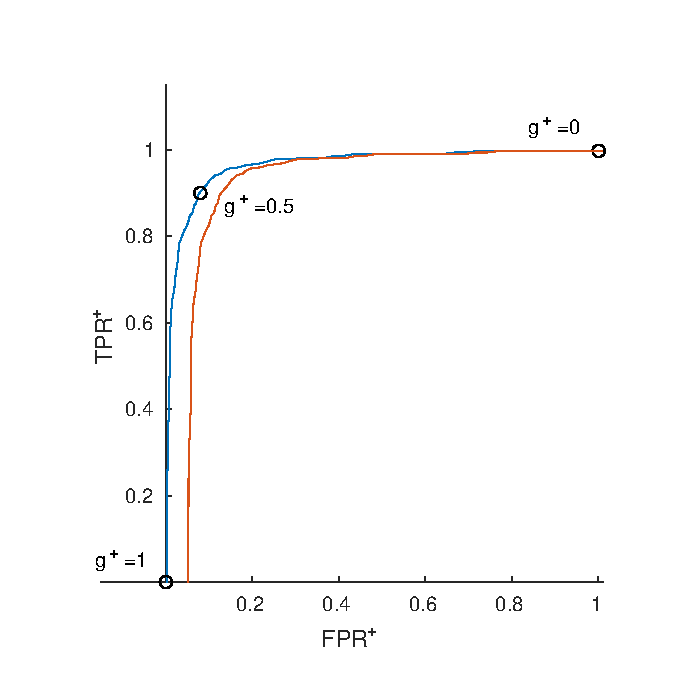
\includegraphics[width=0.5\textwidth]{ros}
    \caption{The ROS curve obtained by test data is depicted in blue, the $\epsilon$-margin for a $\beta$ confidence is shown in red.}
    \label{fig:ros}
\end{figure}

Note, that the rate above correspond to unknown conditional probabilities. E.g.\
$\widehat\FPR(g_l^+)$ represents the expected value of the conditional probability $p( c_l(a)\geq g_l^+ \mid a\in T(l))$.

\subsection{Classifier Optimization}
Let $\Phi$ be a formula that restricts the availability of a maneuver in favor of safety. 
E.g.\ $\Phi$ allows a fast transit of a critical passage only if it can be ensured that there a no humans on the sidewalk. In such a setting $\Phi = l_1 \land \l2 \land \dots \land l_n$ is a conjunction of literals $l_i=\lnot A_i$ of the form ``it is false that there is a human at cell $c_i$''. The truth value of each atom $A_i$ directly depends on a classifier output, which is, in our example, a human classifier. Our goal is to find an optimal threshold values for the related classifiers, separately for each cell,
such that the risk of missperception is restricted to a given safety bound
$\epsilon$ while the availability is maximized.

We want to ensure that the false positive rate of $\Phi$ is below a
given threshold $\epsilon$. Clearly, $\Phi$ is false if at least one literal
is a false positive. On the other hand, $\Phi$ is positive if and only if
all literals are positive. Taking both arguments together yields that
$\Phi$ is a false positive if and only if all literals are false positives.

Recall, that the false positive rates under consideration corresponds
to the expected value of conditional probabilities.
For stochastically independent events we have the identity 
$p(A_1|B_1)\cdot p(A_2|B_2) = p(A_1,A_2|B_1,B_2)$. Under the assumption that
the underlying classifiers of two literals are stochstically independent,
this allows us to represent the false negative rate of a conjunction as the
product of the literals. The same argument holds for the true positive rate.

Hence, we are allowed to distribute a given threshold $\epsilon$ for the
false positive rate of $\Phi$, i.e., $\FPR_\Phi+\epsilon\geq\widehat{\FPR_\Phi}$ to the literals $\prod\epsilon_i = \epsilon$ such that $\epsilon_i$
is an individual threshold for the false positive rate for the literals $l_i$.

%which -- in turn -- finally yields a threshold for the related classifiers, i.e., $\FPR(g^-)+\epsilon_i \geq  \widehat{\FPR(g^-)}$.
%
%Wie bekommen wir jetzt eine Abschätzung für die TP-Rate?
%Wir haben nun $g^-$ möglichst scharf gestellt.
%Wählen wir nun $g^- = g^+$, dann haben wir die Situation, dass wir größer oder gleich
%$g^-$ ist, suchen wir nun eine Einstellung für $g^+$, so dass wir, wenn



%We make the following assumption: 
%Let $c_l$ and $c_{l'}$ be two classifiers, where $l$ is more specific than $l'$. Then
%for quality measure and any thresholds for $c_l$ there exists thresholds for $c_{l'}$ 
%such that $c_{l'}$ is of equal of better quality than $c_l$.

%Before we proceed to give a precise definition of the label assignment of a fused classifier we introduce some additional concepts.
%\begin{itemize}
%\item A set of labels $L=\{l_1,\dots,l_n\}$ is consistent (with respect to the ontology)
%if $\bigsqcap\limits_{l\in L} l \neq \bot$. Otherwise, $L$ is called inconsistent (with %respect to the ontology).
%\item Let $L$ be inconsistent. A subset $L'\subseteq L$ is called a maximal consistent subset of $L$ if $L'$ is consistent and for any $l\in L\setminus L'$ the set $L'\cup\{l\}$ is inconsistent.
%\end{itemize}

We combine several classifiers $c_1,c_2,\dots, c_n$ with upper thresholds $g_1^+, g_2^+, \dots, g_n^+$ and lower thresholds $g_1^-, g_2^-, \dots, g_n^-$ using the vector notion $\mathbf c = (c_1,\dots,c_n)^T$, $\mathbf g^+=(g_1^+,\dots, g_n^+)^T$, $\mathbf g^-=(g_1^-,\dots,g_n^-)^T$. 

For any artifact $a$ we define the auxiliary sets
$P(a) = \{l_i\mid c_i(a) \geq g_i^+\}$ representing positive evidences and
$N(a) = \{\overline{l_i}\mid c_i(a) < g_i^-\}$ representing negative evidences.
The label assignment of the fused classifier is defined as follows
\begin{gather*}
    \mathrm{type}(a,\mathbf c, \mathbf g^+,\mathbf g^-) = 
    \underbrace{
    \bigsqcup\limits_{\substack{\text{$P$ is maximal}\\\text{consistent subset}\\\text{of $P(a)$}}} \bigsqcap\limits_{l \in P} l}_{\text{(A)}}
    \sqcap
    \underbrace{
    \bigsqcup\limits_{\substack{\text{$N$ is maximal}\\\text{consistent subset}\\\text{of $N(a)$}}} \bigsqcap\limits_{l \in N} l}_{\text{(B)}}
    %\bigsqcup\limits_{i\in P(a)} l_i \sqcap \bigsqcap\limits_{i\in N(a)} \overline{l_i},
\end{gather*}
with the convention that the expression $(A)$ evaluates to $\top$ if $P(a)$ is empty.
That is, positive and negative evidence are treated separately at first. 
Then consistent evidence is used to specialize the classification, whereas inconsistent evidence is used to broaden the classification.

\todo[inline]{WH: Ein etwas komplizierteres Beispiel: Wir haben positive Evidenzen Dackel, Katze und negative Evidenz fuer Hund. Die maximal konsistenten Mengen der positiven Evidenzen sind Dackel und Katze, wir bekommen also Tier. Zusammen mit der negativen Evidenz bekommen wir also, dass es sich um  ein Tier handelt, dass kein Hund ist. Macht das Sinn?
\\
Annaehrend. Tatsaechlich wird es sich wohl um eine Katze handeln. Begruendung. Jeder Testdatensatz fuer ein Dackel ist auch Testdatensatz fuer einen Hund. Es gibt mehr Testdatensaetze fuer den Hund. Nach Hoeffding muessen wir also mit mehr Unsicherheiten bei der Dackelklassifikation rechnen. Deshalb koennen wir also davon ausgehen, dass die Aussage kein Hund stimmt. Katze ist mit dieser Aussage konsistent.
\\
Ist dieses Argument valide? Was wir mit Sicherheit sagen koennen, ist dass die Erwartungswerte für den Hundeklassifikator sicherer als die Erwartungserte für den Dackel sind.}

\begin{example}
\begin{table}
$\begin{array}{cc|c}
    (1)&(2)&(3)\\
    \hline
    l_1 &l_2 & l_1 \sqcup l_2\\
    l_1 &\overline{l_2} & l_1\\
    l_1 &\top& l_1\\
    \overline{l_1} &l_2 & l_2\\
    \overline{l_1} &\overline{l_2} & \overline{l_1}\sqcap \overline{l_2}\\
    \overline{l_1} &\top& \overline{l_1}\\
    \top & l_2 & l_2\\
    \top & \overline{l_2} & \overline{l_2}\\
    \top & \top & \top
  \end{array}$
  \quad
  $\begin{array}{cc|c}
    (1)&(2)&(3)\\
    \hline
    l_1 &l_2 & l_1\\
    l_1 &\overline{l_2} & \bot\\
    l_1 &\top & l_1 \\
    \overline{l_1} &l_2 & l_2 \sqcap \overline{l_1}\\
    \overline{l_1} &\overline{l_2} & \overline{l_2}\\
    \overline{l_1} &\top & \overline{l_1}\\
    \top & l_2 & l_2\\
    \top &\overline{l_2} & \overline{l_2}\\
    \top & \top & \top
  \end{array}$
  \caption{ The left table shows the result of joining two classifiers with $l_1 \sqcap l_2=\bot$ and the right table shows the result of joining two classifiers with
  $l_1 \sqsubseteq l_2$.\\ Column (1) shows the result of $\mathrm{type}(a,c_1,g_1^+,g_1^⁻)$,
  column (2) the result of $\mathrm{type}(a,c_2,g_2^+,g_2^⁻)$, and
  column (3) the joined result of $\mathrm{type}(a,\mathbf c, \mathbf g^+, \mathbf g^⁻)$.}
\end{table}

\end{example}

\subsection{Classifier Optimization}
Let $\Phi$ be an Boolean combination of atoms $A_1$, \dots, $A_n$, where the truth value of the atoms depends on classifiers.
Assume $\Phi$ is a safety critical formula, i.e.\ whenever $\Phi$ holds, ego is only allowed to perform safe maneuvers. That is, we have to find optimal thresholds for the classifiers such that $\Phi$ becomes false only in sufficiently secured cases.

The truth value of $\Phi$ is given by the truth values of its atoms. In a first step, we analyze this dependency. A valuation $v$ of the atoms with uncertainties is a function that maps each atom to $0$, $1$ or $?$, where $0$ represents that the atom does not hold, $1$ represents that the atom holds, and $?$ represents that it is not known whether the atom holds or not. The resulting trivalent truth value for $\Phi$ can be computed by exploiting ontological dependencies between the atoms.\todo{Das habe ich zwar geschrieben, wie das im Detail aussieht, weiss ich ehrlich gesagt nicht.}. Since $\Phi$ is only allowed
to become false in sufficiently secured cases, we subsume the cases where 
$\Phi$ is unknown to the cases where $\Phi$ is true. The following table depicts all
valuations for the atoms under which $\Phi$ is true:
\begin{gather*}
  \begin{array}{ccccc|c}
    A_1& A_2 & A_3 & \dots & A_n & \Phi\\
    \hline
    1  &  ?  &    1 & \dots& 0   & 1\\
    1  &  1  &    1 & \dots& 0   & 1\\    
    1  &  ?  &    1 & \dots& 0   & 1\\    
    0  &  0  &    1 & \dots& 1   & 1\\
    \vdots & \vdots & \vdots & \vdots &\vdots & \vdots\\
    ?  &  ?  &    ? & \dots& ?   & 1
  \end{array}
\end{gather*}
There are some atoms $A_i$ for which either $v(A_i)=0$ or $v(A_i)=1$ can lead to a satisfying valuation for $\Phi$. These are exactly those atoms which occure with both polarities in a minimal conjunctive normal form of $\Phi$. For these atoms there is obviously no clear direction of optimization. Hence, we restrict our optimization to atoms occuring with one polarity in the minimal CNF. For simplicity, let us assume that the remaining atoms are of the form $A_i\equiv\textrm{label}(c_l,g_l^+,g_l^-)(a)=l$. Further assume, that $A_i$ occurs in positive polarity. 
That is, we want to assign thresholds $g_l^+$ and $g_l^-$ such that the classifier yields a false negative rate as small as possible while maintaining a sufficient high sensitivity.

\subsection{Adjusting Hoeffding's inequality}












\section{State of Art}\label{sec:relatedwork}
Highly automated vehicles are typically \emph{learning-enabled cyber physical systems} operating in an uncertain dynamic environment, where learning about the \emph{dynamic environment} is enabled through \emph{inaccurate sensors}. This renders an exact inference of the state of the environment infeasible, necessitating suitable representations of the \emph{uncertainty} in such an inference about the dynamic environment. Appropriate representations of uncertainty in the inference have been investigated a.o. within the paradigm of \emph{probabilistic robotics}~\cite{probrob}, particularly as applied to vehicle localization in urban environments~\cite{Thrun2007,Thrun2009,Thrun2010}. In these and related works such as~\cite{Perrolaz2014,moras2014}, the environment uncertainty is represented as \emph{probabilistic
beliefs}. More recently, the challenge of assuring the autonomy of learning-enabled cyber physical systems has been partially addressed in the works~\cite{SeshiaNFM17,SeshiaSadigh18a,SeshiaSasdigh18b}. In particular, \cite{SeshiaNFM17} considers the problem of falsifying signal temporal logic specifications for learning-enabled cyber physical systems, with the technique demonstrated on a simplified model of an automatic emergency braking system with a perception component based on deep neural networks. ``Human-aware'' dynamic control of semi-autonomous vehicles is considered in ~\cite{SeshiaSadigh18a} for estimating (and possibly even changing) the (cognitive) internal state of the human in the loop based on the observed (human) responses, by means of optimal planning through inverse reinforcement learning. A synthesis-based approach, aiming to ensure the correctness of learning-enabled cyber physical systems by construction, starting from probabilistic temporal logic specifications, with applications to autonomous driving under perception uncertainty in adversarial  environments is presented in~\cite{SeshiaSasdigh18b}. Markov Decision Processes form the operational basis of the models in~\cite{Topcu18} generated from reinforcement learning, where strategies conforming to probabilistic temporal logic specifications are synthesized with the aim of enabling the safe navigation of autonomous systems among humans. When viewing the humans in such a setting as \emph{random obstacles}, such safe navigation may be formulated in the operational framework of \emph{stochastic hybrid systems}~\cite{LygerosPrandiniSHS,FraenzleProcosSHS} as a \emph{stochastic reach avoid problem}~\cite{TomlinHSCC2011}, solved by synthesis of stochastic optimal control policies using techniques from dynamic programming. Safe navigation of cooperative driver assistance systems by verification against probabilistic temporal properties has been considered in~\cite{DammMSCS13}. Prediction (using Gaussian propagation)  of the trajectory of motion of an autonomous vehicle  interacting with other traffic agents under uncertainty in localization and control (based on a Linear-Quadratic Gaussian Framework) is considered in~\cite{XuDolanICRA2014}. The related theme of stochastic control of linear systems under Gaussian uncertainty in the environment and in the system's trajectory is addressed in the works~\cite{VitusTomlinCDC2012,VitusTomlinCDC2013}. 








\section{Conclusion}

Werner
0,5 page	concluded at page 15
\bibliographystyle{splncs04}
\bibliography{references.bib}

\end{document}
